%%%%%%%%%%%%%%%%%%%%%%%%%%%%%%%%%%%%%%%%%
% Short Sectioned Assignment LaTeX Template Version 1.0 (5/5/12)
% This template has been downloaded from: http://www.LaTeXTemplates.com
% Original author:  Frits Wenneker (http://www.howtotex.com)
% License: CC BY-NC-SA 3.0 (http://creativecommons.org/licenses/by-nc-sa/3.0/)
%%%%%%%%%%%%%%%%%%%%%%%%%%%%%%%%%%%%%%%%%

%----------------------------------------------------------------------------------------
%	PACKAGES AND OTHER DOCUMENT CONFIGURATIONS
%----------------------------------------------------------------------------------------

\documentclass[paper=a4, fontsize=11pt]{scrartcl} % A4 paper and 11pt font size

% ---- Entrada y salida de texto -----

\usepackage[T1]{fontenc} % Use 8-bit encoding that has 256 glyphs
\usepackage[utf8]{inputenc}
%\usepackage{fourier} % Use the Adobe Utopia font for the document - comment this line to return to the LaTeX default

% ---- Idioma --------

\usepackage[spanish, es-tabla]{babel} % Selecciona el español para palabras introducidas automáticamente, p.ej. "septiembre" en la fecha y especifica que se use la palabra Tabla en vez de Cuadro

% ---- Otros paquetes ----

\usepackage{url} % ,href} %para incluir URLs e hipervínculos dentro del texto (aunque hay que instalar href)
\usepackage{amsmath,amsfonts,amsthm} % Math packages
%\usepackage{graphics,graphicx, floatrow} %para incluir imágenes y notas en las imágenes
\usepackage{graphics,graphicx, float} %para incluir imágenes y colocarlas

% Para hacer tablas comlejas
%\usepackage{multirow}
%\usepackage{threeparttable}

%\usepackage{sectsty} % Allows customizing section commands
%\allsectionsfont{\centering \normalfont\scshape} % Make all sections centered, the default font and small caps

\usepackage{fancyhdr} % Custom headers and footers
\pagestyle{fancyplain} % Makes all pages in the document conform to the custom headers and footers
\fancyhead{} % No page header - if you want one, create it in the same way as the footers below
\fancyfoot[L]{} % Empty left footer
\fancyfoot[C]{} % Empty center footer
\fancyfoot[R]{\thepage} % Page numbering for right footer
\renewcommand{\headrulewidth}{0pt} % Remove header underlines
\renewcommand{\footrulewidth}{0pt} % Remove footer underlines
\setlength{\headheight}{13.6pt} % Customize the height of the header

\numberwithin{equation}{section} % Number equations within sections (i.e. 1.1, 1.2, 2.1, 2.2 instead of 1, 2, 3, 4)
\numberwithin{figure}{section} % Number figures within sections (i.e. 1.1, 1.2, 2.1, 2.2 instead of 1, 2, 3, 4)
\numberwithin{table}{section} % Number tables within sections (i.e. 1.1, 1.2, 2.1, 2.2 instead of 1, 2, 3, 4)

\setlength\parindent{0pt} % Removes all indentation from paragraphs - comment this line for an assignment with lots of text

\newcommand{\horrule}[1]{\rule{\linewidth}{#1}} % Create horizontal rule command with 1 argument of height

\graphicspath{ {./images/} }
\usepackage{subcaption}
\usepackage{hyperref}
\usepackage{soul}


%----------------------------------------------------------------------------------------
%	TÍTULO Y DATOS DEL ALUMNO
%----------------------------------------------------------------------------------------

\title{	
\normalfont \normalsize 
\textsc{\textbf{Aprendizaje Automático (2019)} \\ Doble Grado en Ingeniería Informática y Matemáticas \\ Universidad de Granada} \\ [25pt] % Your university, school and/or department name(s)
\horrule{0.5pt} \\[0.4cm] % Thin top horizontal rule
\huge Memoria Práctica 2 \\ % The assignment title
\horrule{2pt} \\[0.5cm] % Thick bottom horizontal rule
}

\author{Luis Balderas Ruiz \\ \texttt{luisbalderas@correo.ugr.es}} 
 % Nombre y apellidos 


\date{\normalsize\today} % Incluye la fecha actual

%----------------------------------------------------------------------------------------
% DOCUMENTO
%----------------------------------------------------------------------------------------

\begin{document}

\maketitle % Muestra el Título

\newpage %inserta un salto de página

\tableofcontents % para generar el índice de contenidos

\listoffigures

\listoftables

\newpage


%----------------------------------------------------------------------------------------
%	Introducción
%----------------------------------------------------------------------------------------

\section{EJERCICIO SOBRE LA COMPLEJIDAD DE H Y EL RUIDO}

\subsection{Ejercicio 1}

\textbf{Dibujar una gráfica con la nube de puntos de la salida correspondiente:}

\begin{itemize}
	\item[a)] Considere $N=50, dim=2, rango=[-50,50]$ con \textit{simula\_unif}
	
	La ejecución de la función \textit{simula\_unif($50,2,[-50,50]$)} tiene la siguiente salida:
	
	\begin{figure}[H] %con el [H] le obligamos a situar aquí la figura
		\centering
		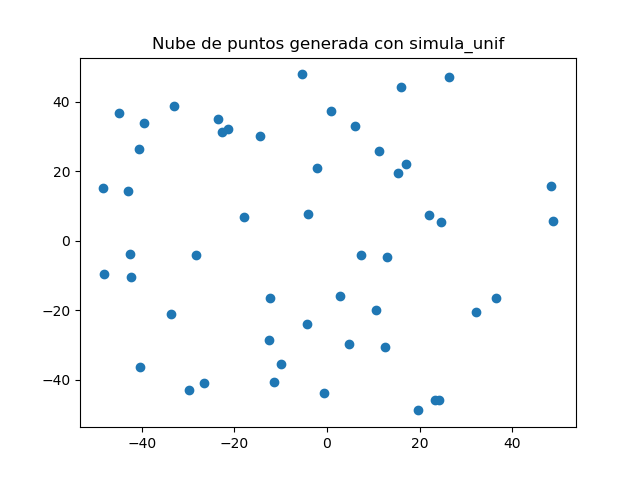
\includegraphics[scale=0.5]{simula_unif1.png}  %el parámetro scale permite agrandar o achicar la imagen. En el nombre de archivo puede especificar directorios
		\caption{Simulación de 50 puntos 2D entre [-50,50] con probabilidad uniforme} 
		\label{fig:simula-unif}
	\end{figure}
	
	\item[b)] Considere $N=50, dim=2, sigma=[5,7]$ con \textit{simula\_gauss}
	La ejecución de la función \textit{simula\_gauss($50,2,[5,7]$)} tiene la siguiente salida:
	
	\begin{figure}[H] %con el [H] le obligamos a situar aquí la figura
		\centering
		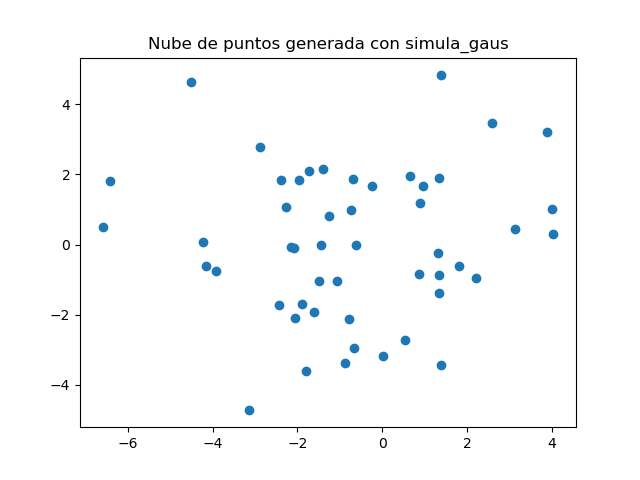
\includegraphics[scale=0.5]{simula_gauss1.png}  %el parámetro scale permite agrandar o achicar la imagen. En el nombre de archivo puede especificar directorios
		\caption{Simulación de 50 puntos 2D de una gaussiana con desviación típica entre [5,7]} 
		\label{fig:simula-gauss}
	\end{figure}
\end{itemize}

\subsection{Ejercicio 2}

\textbf{Con ayuda de la función \textit{simula\_unif()}} generar una muestra de puntos 2D a los que vamos a añadir una etiqueta usando el signo de la función $f(x,y) = y -ax-b$, es decir, el signo de la distancia a cada punto a la recta simulada con \textit{simula\_recta()}

\begin{itemize}
	\item[a)] Dibujar una gráfica donde los puntos muestren el resultado de su etiqueta, junto con la recta usada para ello.
	
	Creo una recta aleatoria con la función \textit{simula\_recta()} de forma que su pendiente y su ordenada en el origen son las siguientes:
	
	$$a = -2.04013210695, b=-46.0760383842$$
	
	Tras generar el dataset de 50 puntos, etiqueto cada uno de ellos en función de si están por encima o por debajo de la recta (cada color indica una situación). El resultado es el siguiente: 
	
	\begin{figure}[H] %con el [H] le obligamos a situar aquí la figura
		\centering
		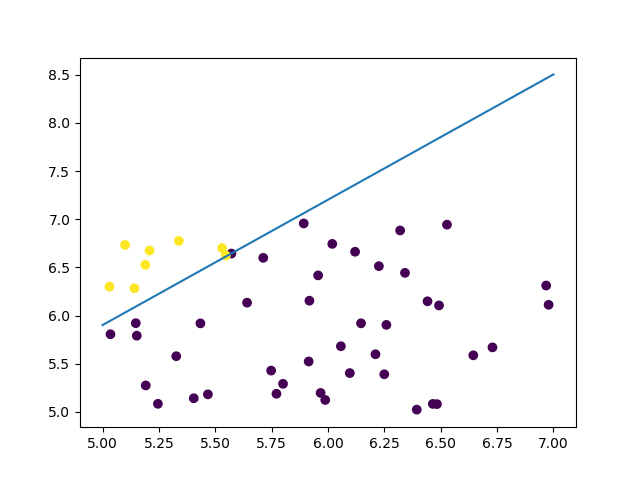
\includegraphics[scale=0.5]{recta1.png}  %el parámetro scale permite agrandar o achicar la imagen. En el nombre de archivo puede especificar directorios
		\caption{Plot de los 50 datos generados uniformemente y la recta aleatoria que los separa en dos partes} 
		\label{fig:recta1}
	\end{figure}

Como se puede ver, todos los puntos están bien clasificados.

	\item[b)] Modifique de forma aleatoria un $10\%$ etiquetas positivas y otro en negativas y guarde los puntos con sus nuevas etiquetas. Dibuje de nuevo la gráfica anterior.
	
	El resultado de esta modificación aleatoria depende mucho de dónde se situó la recta en el apartado anterior. Las dos clases de puntos están desbalanceadas por lo que se verá que una de ellas se cambian menos puntos que la otra. Sin embargo, se garantiza que son el $10\%$ (redondeando a la baja). Veamos el resultado:
	
	\begin{figure}[H] %con el [H] le obligamos a situar aquí la figura
		\centering
		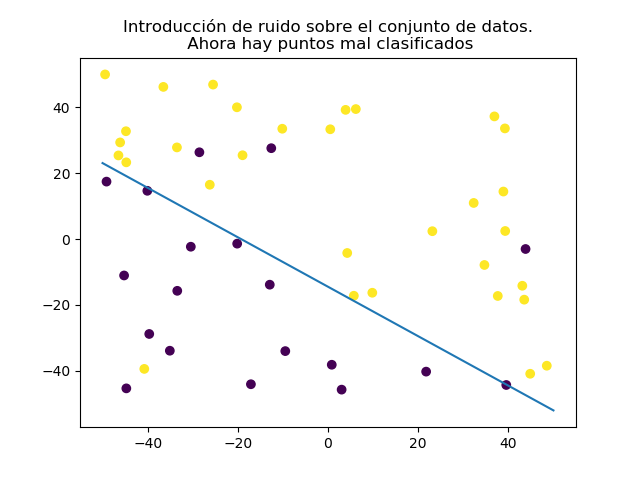
\includegraphics[scale=0.5]{recta2.png}  %el parámetro scale permite agrandar o achicar la imagen. En el nombre de archivo puede especificar directorios
		\caption{Introducción de ruido en el dataset anterior} 
		\label{fig:recta2}
	\end{figure}

Como se puede ver, hay 4 puntos mal clasificados y hemos conseguido que el conjunto no sea linealmente separable.
\end{itemize}

\subsection{Ejercicio 3}

\textbf{Supongamos ahora que las siguientes funciones definen la frontera de clasificación de los puntos de la muestra en lugar de una recta. Visualizar el etiquetado generado en 2b junto con cada una de las gráficas de cada una de las funciones. Comparar las formas de las regiones positivas y negativas de estas nuevas 	funciones con las obtenidas en el caso de la recta ¿Son estas funciones más complejas	mejores clasificadores que la función lineal? ¿En que ganan a la función lineal? Explicar el razonamiento}



\begin{itemize}
	\item $f(x,y) = (x-10)^2+(y-20)^2-400$
	
	\begin{figure}[H] %con el [H] le obligamos a situar aquí la figura
		\centering
		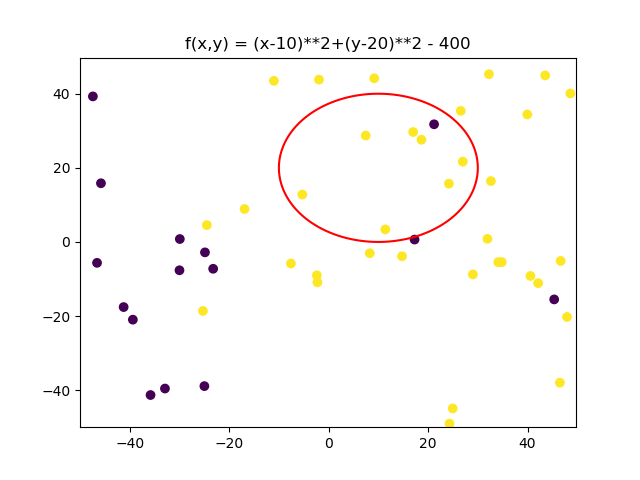
\includegraphics[scale=0.5]{f1.png}  %el parámetro scale permite agrandar o achicar la imagen. En el nombre de archivo puede especificar directorios
		\caption{$f(x,y) = (x-10)^2+(y-20)^2-400$ con los puntos de 2b} 
		\label{fig:f1}
	\end{figure}

Como se puede ver, esta función no sirve para separar las dos clases. La lineal del ejercicio anterior, aunque tiene cuatro errores, separa mucho mejor.

\item $f(x,y) = 0.5(x+10)^2+(y-20)^2-400$
\begin{figure}[H] %con el [H] le obligamos a situar aquí la figura
	\centering
	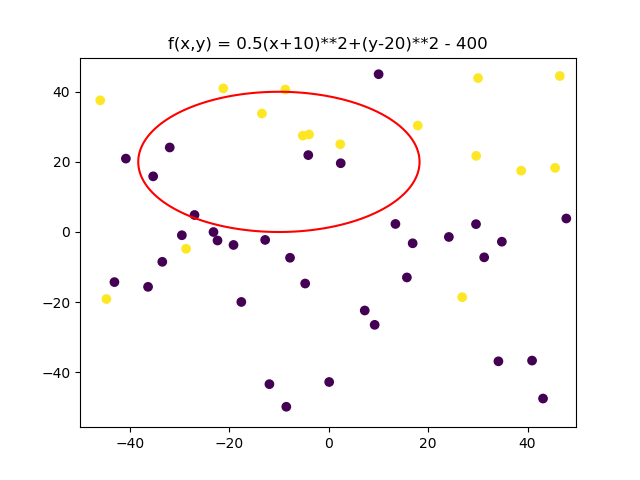
\includegraphics[scale=0.5]{f2.png}  %el parámetro scale permite agrandar o achicar la imagen. En el nombre de archivo puede especificar directorios
	\caption{$f(x,y) = 0.5(x+10)^2+(y-20)^2-400$ con los puntos de 2b} 
	\label{fig:f2}
\end{figure}

De nuevo, se puede ver que no es una función propicia para separar los datos de 2b. No se consigue ninguna ventaja respecto de la recta.

\item $f(x,y) = 0.5(x-10)^2-(y+20)^2-400$
\begin{figure}[H] %con el [H] le obligamos a situar aquí la figura
	\centering
	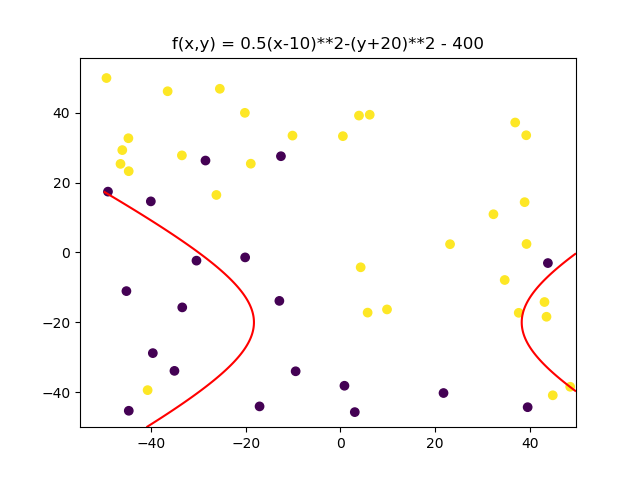
\includegraphics[scale=0.5]{f3.png}  %el parámetro scale permite agrandar o achicar la imagen. En el nombre de archivo puede especificar directorios
	\caption{$f(x,y) = 0.5(x-10)^2-(y+20)^2-400$ con los puntos de 2b} 
	\label{fig:f3}
\end{figure}

Esta hipérbola consigue dejar a derecha izquierda dos clases distintas pero los puntos que se quedan entre medias de las ramas no tienen ninguna separación. Por tanto, tampoco hay ganancia con respecto a la recta.

\item $f(x,y) =  y -20x^2-5x+3$

En este caso, la parábola es la peor función hasta el momento para separar los datos. Veamos:

\begin{figure}[H] %con el [H] le obligamos a situar aquí la figura
	\centering
	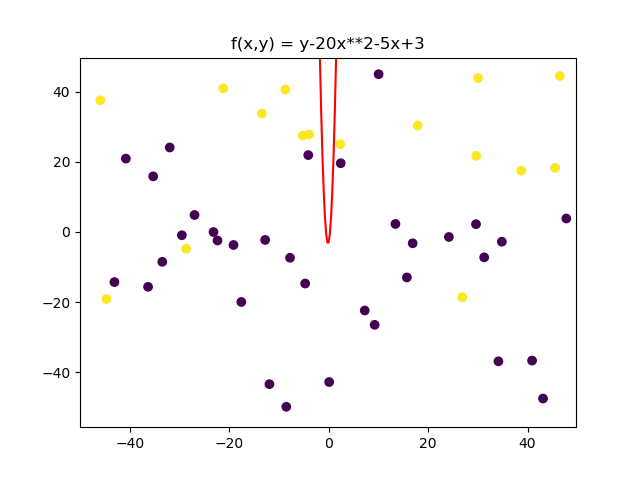
\includegraphics[scale=0.5]{f4.png}  %el parámetro scale permite agrandar o achicar la imagen. En el nombre de archivo puede especificar directorios
	\caption{$f(x,y) =  y -20x^2-5x+3$ con los puntos de 2b} 
	\label{fig:f4}
\end{figure}

Está claro que no genera ningún beneficio en este caso con respecto a la recta.

\end{itemize}

Como se puede ver, ninguna modificación compleja de la función lineal original ha servido para mejorar la clasificación. El motivo es que los datos son prácticamente linealmente separables (solamente han cambiado las etiquetas de 4 puntos) por lo que, a pesar de que no clasificaría el 100\% de los datos bien, comete un error muy pequeño.


\section{MODELOS LINEALES}

\subsection{Ejercicio 1}

\textbf{Implementar la función ajusta\_PLA que calcula el hiperplano solución a un problema de clasificación binaria usando el algoritmo PLA. La función devuelve los coeficientes del hiperplano}

\begin{itemize}
	\item[a)] Ejecutar el algoritmo PLA con los datos simulados en los apartados 2a. Inicializar el algoritmo con: a) el vector cero y, b) con vectores de números aleatorios en [0,1] (10 veces). Anotar el número medio de iteraciones necesarias en ambos para converger. Valorar el resultado relacionando el punto de inicio con el número de iteraciones.
	
	En el primer caso, con un vector cero, los resultados son constantes. Los resultados son los siguientes:
	
	 w =  (334,13.38587411,4.62931342) y 55 iteraciones de media. He aquí el ajuste:
	
	\begin{figure}[H] %con el [H] le obligamos a situar aquí la figura
		\centering
		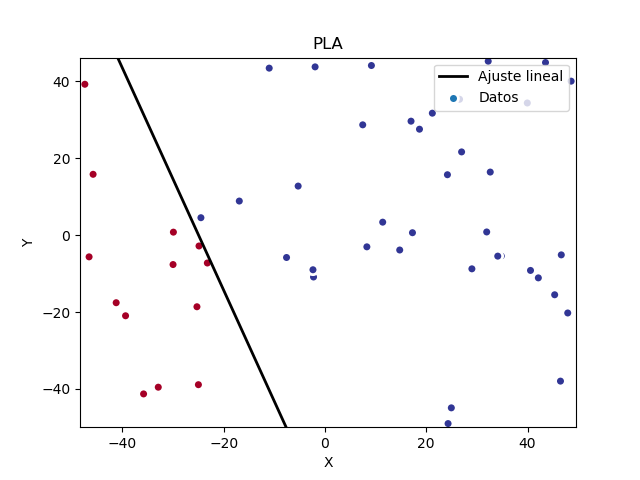
\includegraphics[scale=0.5]{PLA1.png}  %el parámetro scale permite agrandar o achicar la imagen. En el nombre de archivo puede especificar directorios
		\caption{Ajuste de PLA con para los datos de 2a inicializado con vector cero} 
		\label{fig:pla1}
	\end{figure}

	En el segundo caso, con un vector inicializado con números aleatorios entre 0 y 1, se obtienen los siguientes resultados (w varía en función de la iteración): 53.4 iteraciones de media para la convergencia. Por mostrar que funciona de manera conveniente, represento el resultado de la primera iteración:
	
	\begin{figure}[H] %con el [H] le obligamos a situar aquí la figura
		\centering
		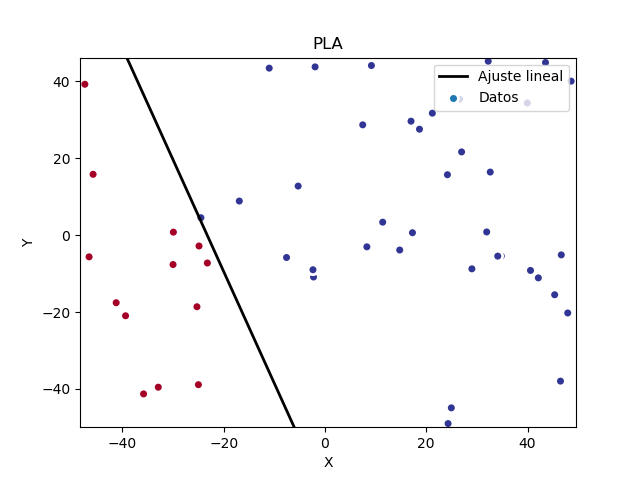
\includegraphics[scale=0.5]{PLA2.png}  %el parámetro scale permite agrandar o achicar la imagen. En el nombre de archivo puede especificar directorios
		\caption{Ajuste de PLA con para los datos de 2a inicializado con vector aleatorio} 
		\label{fig:pla2}
	\end{figure}
	
	\item[b)] Hacer lo mismo que antes usando ahora los datos del apartado 2b. ¿Observa algún comportamiento diferente? En caso afirmativo diga cuál y las razones para que ello ocurra.
	
	Efectivamente, el comportamiento es diferente. Los datos generados en el apartado 2b de la sección 1 están caracterizados por la existencia de ruido en ellos. En concreto, de un 10\% de las etiquetas de cada clase. Por tanto, el conjunto de datos no es linealmente separable. En consecuencia, el algoritmo PLA no puede converger y generar un hiperplano (una recta en este caso) que separe los datos \cite{lfd}, \cite{esl}. 
	
	Como se puede ver en la ejecución del algoritmo, tras 15000 iteraciones, los resultados son distintos cada vez y no se consigue la separación como se puede ver a continuación:
	
	
	\begin{figure}[H] %con el [H] le obligamos a situar aquí la figura
		\centering
		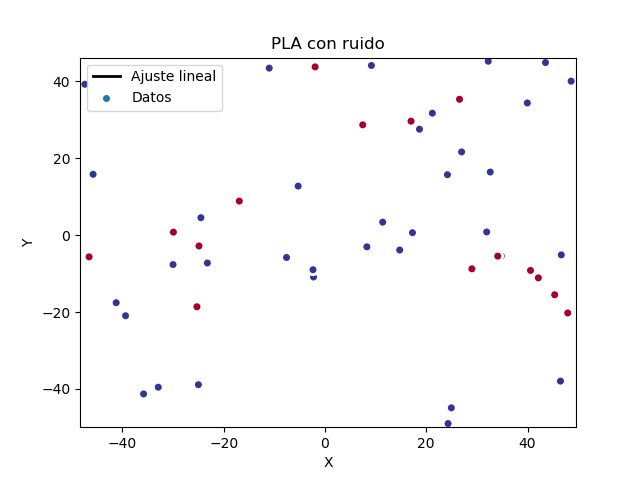
\includegraphics[scale=0.5]{PLA-ruido.png}  %el parámetro scale permite agrandar o achicar la imagen. En el nombre de archivo puede especificar directorios
		\caption{Ajuste de PLA con para los datos de 2b. No hay convergencia} 
		\label{fig:pla-ruido}
	\end{figure}

	Por tanto, sea cual sea el $w$ de inicio, cero o aleatorio, no se alcanza un resultado ni convergencia (la recta se queda fuera de los márgenes previstos en los puntos).
\end{itemize}


\subsection{Ejercicio 2}

\textbf{Regresión Logística}

\begin{itemize}
	\item[a)] Implementar Regresión Logística con SGD bajo las siguientes condiciones: Inicializar el vector de pesos con valores 0; criterio de parada con $\epsilon = 0.01$; aplicar permutación aleatoria antes de cada época; tasa de aprendizaje de $\eta = 0.01$.
	
	En primer lugar, genero el conjunto de datos como se pide, una recta y divido el dataset en dos tipos:
	
	\begin{figure}[H] %con el [H] le obligamos a situar aquí la figura
		\centering
		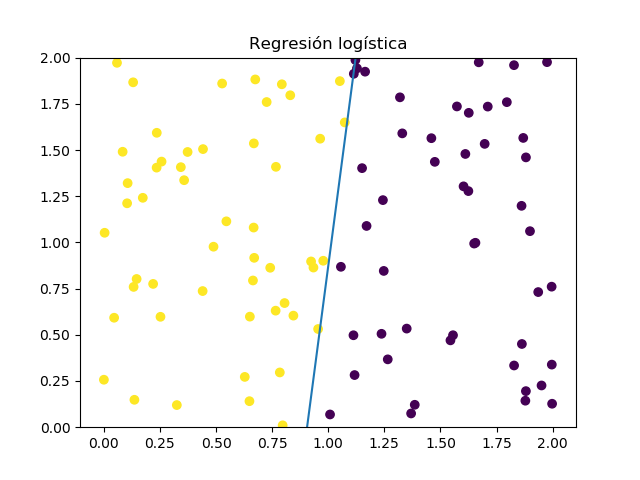
\includegraphics[scale=0.6]{reg-log.png}  %el parámetro scale permite agrandar o achicar la imagen. En el nombre de archivo puede especificar directorios
		\caption{Dataset a evaluar con SGD-RL} 
		\label{fig:reg-log}
	\end{figure}
	
	
	En el archivo de código está implementada la Regresión Logística con SGD. Cabe destacar que es parecida a SGD que desarrollamos en la práctica anterior, teniendo en cuenta que el tamaño del minibatch es 1. Sin embargo, calculamos el gradiente de $E_in$ vía la fórmula de regresión logística:
	$$\nabla E_{in} = \frac{-1}{N} \sum_{n=1}^{N} = \frac{y_n x_n}{1+ e^{y_n w^T(t)x_n}}$$
	
	Muestro ahora el resultado de la ejecución:
	
	w = (-10.69386455, 3.26264871, 6.14173663), $E_{in}$ = 0.13625555
	
	\begin{figure}[H] %con el [H] le obligamos a situar aquí la figura
		\centering
		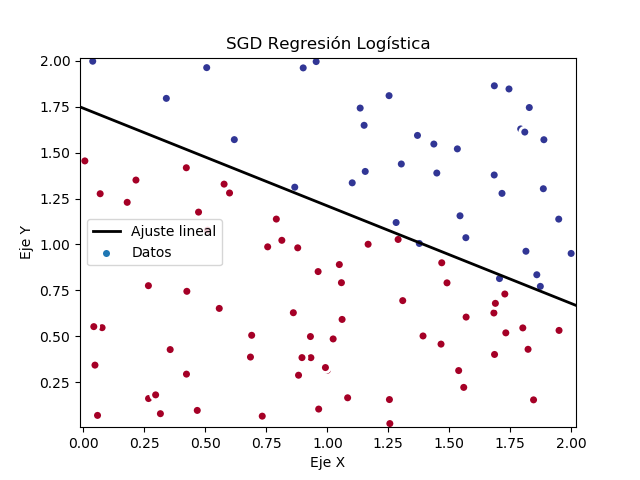
\includegraphics[scale=0.6]{SGD-RL.png}  %el parámetro scale permite agrandar o achicar la imagen. En el nombre de archivo puede especificar directorios
		\caption{SGD-Regresión Logística en training} 
		\label{fig:sgd-rl-train}
	\end{figure}

	\item[b)] Usar la muestra de datos etiquetada para enconrar nuestra solución g y estimar $E_{out}$ usando para ello un número suficientemente grande de datos.
	
	Para este apartado, genero 2000 puntos 2D en $[0,2]\times[0,2]$. Calculo sus etiquetas y obtengo los siguientes resultados:
	
	$E_{out}$ = 0.13496952
	
	\begin{figure}[H] %con el [H] le obligamos a situar aquí la figura
		\centering
		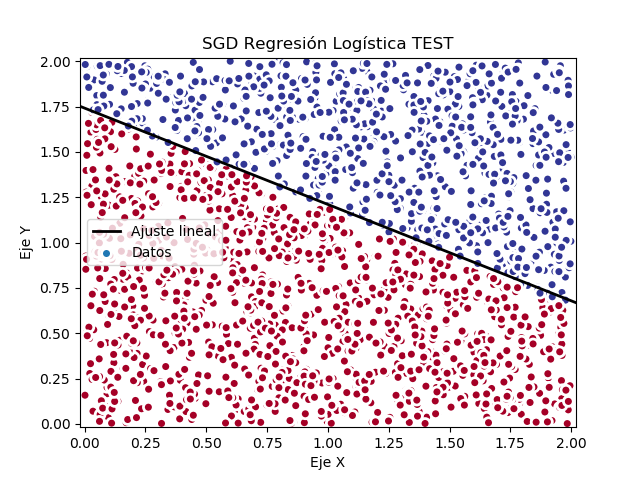
\includegraphics[scale=0.6]{SGD-RL-T.png}  %el parámetro scale permite agrandar o achicar la imagen. En el nombre de archivo puede especificar directorios
		\caption{SGD-Regresión Logística en test} 
		\label{fig:sgd-rl-test}
	\end{figure}
	
	Como se puede comprobar, $E_{out} < E_{in}$. Paradójicamente, en este problema tiene sentido. Si la frontera de decisión es fija (la recta se genera al principio y no se mueve) y simulamos las etiquetas de acuerdo a esa recta, ahora tenemos un dataset a evaluar con una distribución uniforme mucho más poblada que antes. Como SGD-RL ha sido capaz de ajustarse mucho a la frontera de decisión, separa muchísimos más datos  que antes (el dataset es mucho mayor) correctamente y deja prácticamente los mismos mal clasificados, por lo que el error disminuye.
\end{itemize}	
	
\section{BONUS}

\subsection{Ejercicio 1}

\textbf{Considera el conjunto de datos de los dígitos manuscritos. Plantear un problema de clasificación binaria que considere el conjunto de entrenamiento como datos de entrada para aprender la función g. Usar un modelo de Regresión Lineal y aplicar PLA-Pocket como mejora. Responder a la siguientes cuestiones}

\begin{itemize}
	\item[a)] Generar gráficos separados de los datos de entrenamiento y test junto con la función estimada.
	
	En primer lugar, he utilizado la Pseudoinversa como modelo de regresión lineal, ya que lo teníamos implementado en la práctica anterior. Aprovechando Pseudoinversa, el calculado la $w_{ini}$ = (0.50676351, -8.25119739, -0.44464113) . A continuación, con esa $w_{ini}$, ejecuto PLA-Pocket y se obtienen los siguiente resultados:
	
	$w$ = (6.50676351, -94.33278003, -4.88432863)
	
	\begin{figure}[H] %con el [H] le obligamos a situar aquí la figura
		\centering
		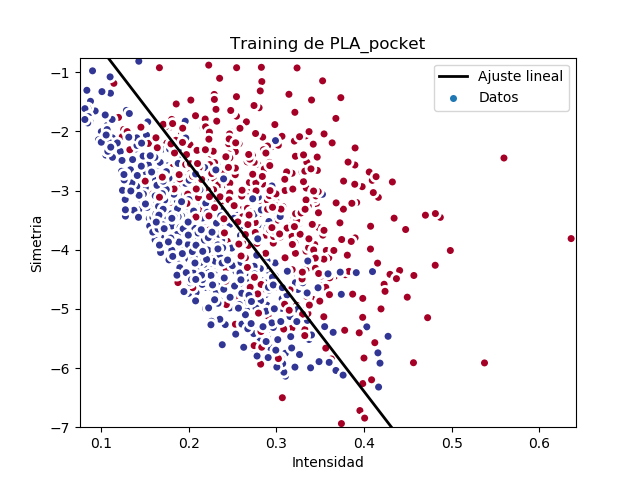
\includegraphics[scale=0.6]{train_pla_pocket.png}  %el parámetro scale permite agrandar o achicar la imagen. En el nombre de archivo puede especificar directorios
		\caption{Resultado de entrenamiento PLA-Pocket+Pseudoinversa} 
		\label{fig:train-pla-pocket}
	\end{figure}

	En el caso de test, el resultado es el siguiente:
	
	\begin{figure}[H] %con el [H] le obligamos a situar aquí la figura
		\centering
		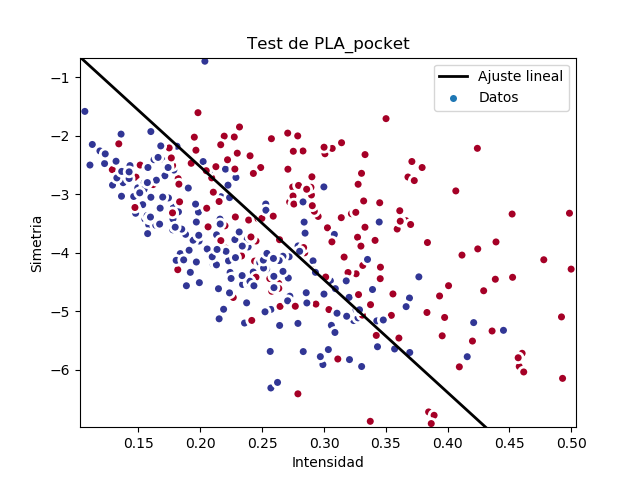
\includegraphics[scale=0.6]{test_pla_pocket.png}  %el parámetro scale permite agrandar o achicar la imagen. En el nombre de archivo puede especificar directorios
		\caption{Resultado de test PLA-Pocket+Pseudoinversa} 
		\label{fig:test-pla-pocket}
	\end{figure}

 	\item[b)] Calcular $E_{in}$ y $E_{test}$
 	
 	Tras realizar los cálculos, vemos los siguientes resultados:
 	
 	$$E_{in} = 0.22529313232830822$$
 	$$E_{test} = 0.2540983606557377$$
 	
 	\item[c)] Obtener cotas sobre el verdadero valor de  $E_{out}$.
 	
 	Pueden calcularse dos cotas (\cite{lfd}). Trato primera la de $E_{in}$. 
 	Sea $h \in H$, fija, $f(x)$ la función objetivo (desconocida), $D$ el conjunto de entrenamiento de tamaño N. Podemos escribir la desigualdad de Hoeffding como sigue:
 	
 	$$P(D: |E_{out}(h)-E_{in}(h)|> \epsilon) \leq 2 e^{-2\epsilon^2N} \hspace{0.5cm} \forall \epsilon > 0$$
 	
 	Llamando $\delta = 2e^{-2\epsilon^2 N}$, tenemos
	
	$$P(D: |E_{out}(h)-E_{in}(h)|> \epsilon) \leq \delta \Rightarrow P(D: |E_{out}(h)-E_{in}(h)| < \epsilon) \geq 1 - \delta$$
	
	Podemos escribir, por tanto, la siguiente desigualdad:
	
	$$E_{out}(h) \leq E_{in}(h) + \sqrt{\frac{1}{2N} \log \frac{2}{\delta}}$$
	con probabilidad al menos $1-\delta$ en $D$.
	
	Considerando una clase de funciones finita, la expresión se convierte en 
	$$E_{out}(h) \leq E_{in}(h) + \sqrt{\frac{1}{2N} \log \frac{2|H|}{\delta}}$$
	
	Sin embargo, el tamaño de la clase de funciones ahora entra en juego y puede hacer menos útil la cota. Para poder garantizar una buena cota, surge la teoría de la generalización y la Dimensión de Vapnik-Chervonenkis (VC). Como se trata de un modelo lineal, VC = 3 y la cota a utilizar es la siguiente:
	
	$$E_{out}(h) \leq E_{in}(h) + \sqrt{\frac{8}{N} \log \frac{4((2N)^{d {VC}}+1)}{\delta}}$$
	
	La cota, por tanto, es $E_{out} \leq 0.656229637799$.
	
	Para el caso de $E_{test}$, cuando afirmamos que $E_{test}$ es un estimador de $E_{out}$, estamos afirmando que $E_{test}$ generaliza muy bien $E_{out}$. En el caso anterior, intentábamos buscar la función que minimizaba $E_{in}$. Ahora, sin embargo, ya tenemos una función fija y queremos simplemente estimar el error. Por tanto, la desigualdad de Hoeffding con una hipótesis es suficiente para el caso de conjunto de test. 
	
	$$E_{out}(h) \leq E_{test}(h) + \sqrt{\frac{1}{2N} \log \frac{2}{\delta}}$$
	
	La cota, por tanto, es $E_{out} \leq 0.325087464088$
	
	Como intentamos minimizar $E_{out}$, la mejor cota es la menor, es decir, la que genera $E_{test}$.
\end{itemize}

\newpage
\section{Bibliografía}

%------------------------------------------------

\bibliography{citas} %archivo citas.bib que contiene las entradas 
\bibliographystyle{plain} % hay varias formas de citar

\end{document}
